\subsection{Gillespie Algorithm}
The Chemical Master Equation presented in the previous chapter gives an exact description of the time evolution of a chemical reaction system. In practice, however, it is impractical (or even impossible) to obtain the solve explicitly. Since it is based on the same basic assumptions, the Gillespie Algorithm is a simulation method that is equivalent to the CME. However, the approach does not try to solve the equation explicitly, but simulates the underlying Markov process the CME describes analytically. The main idea of the algorithm can be summarized by two questions that have to be answered in every simulation step: "What is the next reaction that takes fires?" (i.e.\ what is the next state of the system) and "When will this happen?" (i.e.\ at what time will the state transition take place). In the following the Gillespie SSA will be derived based on basic probability theory concepts. 

Let there be a chemical reaction system with species $X_i$, $i=1, \ldots,N$ and reactions $R_j$, $j=1, \ldots,M$. The state of the system $\vec{x}(t)$ at time $t$ is determined by the number of particles $x_i$ of the species $X_i$. The initial state of the system at time $t_0$ is $\vec{x}_0 = \vec{x}(t_0)$. The state change vector $\vec{\nu_j}$ of reaction $R_j$ is defined such that when the reaction takes place, the state of the system changes from $\vec{x}$ to $\vec{x} + \vec{\nu}_j$. The $i$-th component of the state change vector gives the number of particles that are consumed ($\nu_{ij} < 0$) or created ($\nu_{ij} > 0$) when reaction $R_j$ occurs. In the following derivation, for the sake of readability, the dependency of the propensity functions $\alpha_j$ on the state of the system $\vec{x}(t)$ will be omitted.

For the moment, just a single reaction $R_j$ of the system equipped with the propensity function $\alpha_j$ is considered. Let $f_{0,j}(\tau+d\tau)$ be the probability that the reaction does not fire in the time interval $\lbrack t,t+\tau+d\tau)$, where $d\tau$ is an infinitesimal time step and $\tau > 0$. This is equivalent to the formulation that $R_j$ does not occur in the interval $\lbrack t,t+\tau)$ and in the subsequent instant $(t+\tau+d\tau)$:
\begin{align}
f_{0,j}(\tau + d\tau) = f_{0,j}(\tau) \cdot (1-\alpha_j d\tau). 
\end{align}
Rearranging and passing the limit of $d\tau \to 0$ leads to
\begin{align}
\lim_{d\tau \to 0} \frac{f_{0,j}(\tau + d\tau) - f_{0,j}(\tau)}{d\tau} = \frac{df_{0,j}(\tau)}{d\tau} = -\alpha_j f_{0,j}(\tau)
\end{align}
Solving the differential equation with the initial condition $f_{0,j}(0) = 1$ yields
\begin{align}
\label{eq:probnot}
f_{0,j}(\tau) = \exp(-\alpha_j \tau)
\end{align}

Considering the complete system, in the case that none of the $M$ reactions of the system fires in the interval $\lbrack t,t + \tau)$, one has
\begin{align}
\begin{split}
f_0(\tau) &= \mathcal{P}(\tau_1 > \tau \wedge \tau_2 > \tau \wedge \ldots \wedge \tau_M > \tau) \\ 
&= \mathcal{P}(\min (\tau_j) > \tau) = \prod_{k=1}^M \alpha_k\exp(-\alpha_k \tau) \\ 
&= \exp(-\alpha_0 \tau)
\end{split}
\end{align}
where $\alpha_0 = \sum_{k=1}^M \alpha_k$. 

The probability density $f_1(\tau)$ that any reaction fires at time $t+\tau$ is given by the probability that none fired in the interval $\lbrack t,t+\tau)$ and the probability that exactly one fires in the instant $(t+\tau)$:
\begin{align}
f_1(\tau) = \exp(-\alpha_0 \tau) \cdot \alpha_0
\end{align}
The waiting time $\tau$ until any reaction $R_j$, $j=1,\ldots,M$ fires is therefore exponentially distributed, i.e.\ $\tau \sim \operatorname{Exp}(\alpha_0)$. The corresponding cumulative distribution function (CDF) is given by
\begin{align}
F(\tau) = \int_0^\tau f_1(t) dt = 1 - \exp(-\alpha_0 \tau)
\end{align}
Since most random number generators can only generate random numbers $r_1 \sim \operatorname{Unif}(0,1)$, inverse probability integral transform (cite the paper!!!) can be used to generate $\tau \sim \operatorname{Exp}(\alpha_0)$:
\begin{align}
\tau = F^{-1}(r_1) = \frac{1}{\alpha_0} \ln\left(\frac{1}{1-r_1}\right)
\end{align}
In this case, the (excluded) values $r_1=0$ and $r_1 = 1$ are mapped to $\tau = 0$ and $\tau = \infty$, respectively. A computationally favorable but otherwise equivalent mapping is
\begin{align}
\tau = \frac{1}{\alpha_0} \ln \left( \frac{1}{r_1} \right)
\end{align}
where $r_1=0$ and $r_1=1$ are mapped to $\tau = \infty$ and $\tau = 0$. Considering only the real part of the complex logarithm, it can be obtained by moving the original function to the left by $1$ (i.e.\ $r'=r+1$) and then mirroring it on the ordinate axis. Figure \ref{fig:inversetransform} illustrates this process. 
\begin{figure}
\centering
\includegraphics[width=\textwidth]{images/inversetransform.eps}
\caption{Inverse probability integral transform: original mapping drawn in blue, modified function in red. Solid lines are used in the domain of interest, dashed ones illustrate the symmetry of the function (imaginary parts omited). Asymptotes are indicated by dots.}
\label{fig:inversetransform}
\end{figure}

Now that a way to find the time $\tau$ when the next reaction takes place has been derived, the next step is to determine which reaction actually fired. This, however, is straightforward: 

Let $r_2$ be a random number uniformly distributed in the interval $(0,1)$, i.e.\ $r_2 \sim \operatorname{Unif}(0,1)$. Then $R_j$ is the reaction which fired in the interval $\lbrack t,t+\tau)$ if the index $j$ fulfills
\begin{align}
\label{eq:nextr}
\frac{1}{\alpha_0} \sum_{k=1}^{j-1} \alpha_k \leq r_2 < \frac{1}{\alpha_0} \sum_{k=1}^{j} \alpha_k
\end{align}

Combining the results from above, the Gillespie Algorithm can be outlined as follows: \\
\begin{framed}
\begin{algorithm}[H]
\DontPrintSemicolon
\KwIn{Initial state $\vec{x}_0$, propensity functions $\alpha_j$, time $t_{end}$}
\KwOut{State $\vec{x}(t)$ for $t \in \lbrack t,t_{end}\rbrack$}
 \textbf{Initialization:} Set time $t = 0$ and state $\vec{x} = \vec{x}_0$.\;
 \While{$t < t_{end}$}{
  Generate random numbers $r_1,r_2 \sim \mathcal{U}(0,1)$.\;
  \For{$j = 1$ \KwTo $M$}
  {
  Compute the propensity function $\alpha_j(\vec{x})$.\;
  }
  Compute the sum of all propensities $\alpha_0 = \sum_{j=1}^M \alpha_j$.\;
  Compute the time step $\tau = \frac{1}{\alpha_0} \ln \left( \frac{1}{r_1} \right)$.\;
  Find $j \in \lbrack1,M\rbrack$ such that $\sum_{k=1}^{j-1} \alpha_k \leq r_2 \alpha_0 < \sum_{k=1}^j \alpha_k$ holds.\;
  Set $\vec{x} = \vec{x} + \vec{\nu}_j$.\;
  Set $t = t + \tau$.\;
 }
 \caption{Gillespie Algorithm}
\end{algorithm}
\end{framed}

Figure \ref{fig:gs_time_evolution} shows three independent Gillespie SSA samplings of the temporal evolution of the well-stirred Gray-Scott model. The number of molecules is rescaled to obtain concentrations, the factor $\Omega = 1000$ was used (see chapter \ref{ch:scaling}). Reaction constants are $F=0.04$, $\kappa = 0.06$ and $\rho_s = 2.0$. The initial condition is given as $u_0=500$ and $v_0 = 250$ which is equivalent to initial concentrations of 0.5 and 0.25, respectively. The dashed line indicates the deterministic solution obtained numerically using a fifth-order Runge-Kutta scheme. In Figure \ref{fig:gs_hist_10} a histogram of the number of U molecules at time $t=10$ is shown. The results from 100000 samples are partitioned in 30 bins. 

\begin{figure}
\centering
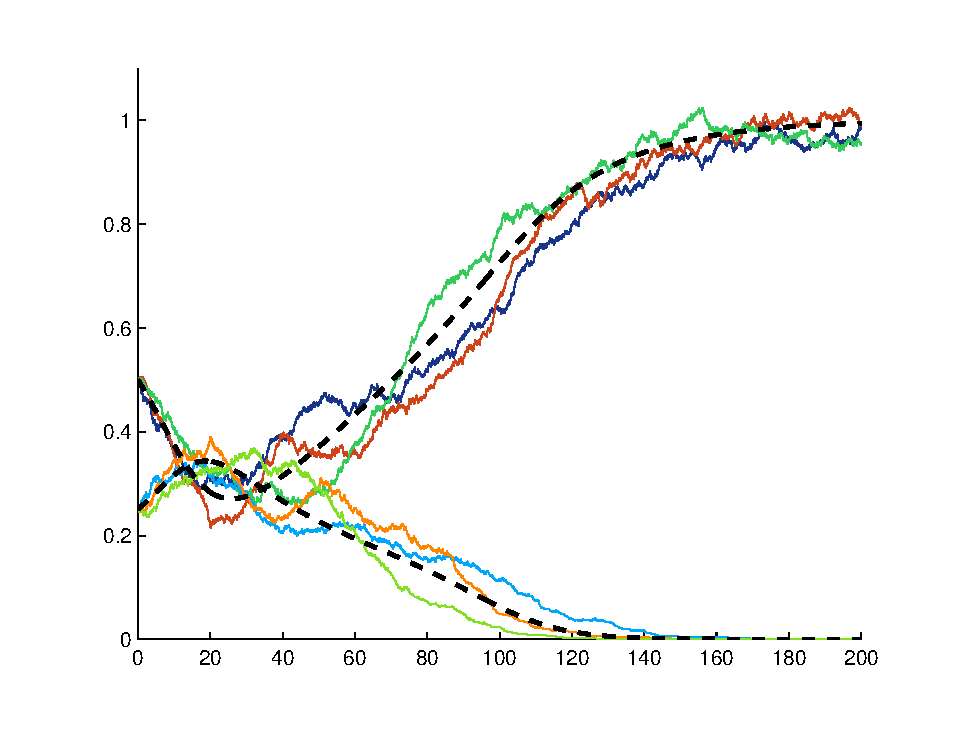
\includegraphics[width=\textwidth]{images/gs_time_evolution.eps}
\caption{Stochastic simulation of the well-stirred Gray-Scott model with $F=0.04$, $\kappa=0.06$, $\rho_s = 2.0$, $u_0=500$ and $v_0=250$. The concentrations ($\Omega=1000$) of both species over times ($t\in[0,200]$)is plotted. Color codeing: dark colors represent species U, bright colors represent species V.}
\label{fig:gs_time_evolution}
\end{figure}

\begin{figure}
\centering
\includegraphics[width=\textwidth]{images/gs_hist_10.eps}
\caption{Histogram obtained by 100000 Gillespie SSA samples evaluated at $t=10$. Parameters and initial conditions similar to figure \ref{fig:gs_time_evolution}}
\label{fig:gs_hist_10}
\end{figure}

\ifdebug
Algorithm (derivation from Oxford Paper)
Leaping condition, tau formula\cite{cao_adaptive_2007}
\begin{itemize}
\item Exact method
\item you can compare time evolution of concentration/number of a specie from deterministic and stochastic simulation 
\item often mean of stochastic realization correspond to deterministic solution, but it is not a rule, but it is nice to show that in the limit of large number of molecules stochastic solution converge to deterministic one
\item A lot of improvements were proposed but it is still computational expensive/prohibitive. 
\end{itemize}
\fi